\section{Theorie}
\label{sec:Theorie}

Ziel des Versuches ist es, Elastizitätsmodule verschiedener Materialen
zu ermitteln, indem die Biegung elastischer Stäbe untersucht wird.

\subsection{Die Spannung an elastischen Körpern}

Die physikalische Größe der mechanischen Spannung $\sigma_m$ ist die wirkende
Kraft $F$ pro Fläche $A$. Sie setzt sich zusammen aus der Normalspannung $\sigma$,
die senkrecht zur Oberfläche wirkt und einer tangential zur Fläche wirkenden
Tangentialspannung.

Spannungen können an Körpern zu Gestalt- und Volumenveränderungen
führen. Liegt durch Druck oder Zug eine Spannung nur in einer Körperdimension vor, 
so ist sie proportional zur Längenänderung $\frac{\Delta L}{L}$ und es ergibt sich
das Hooksche Gesetz

\begin{equation*}
    \sigma = E \cdot \frac{\Delta L}{L}
\end{equation*}

mit dem materialspezifischen Elastizitätsmodul $E$ als Proportionalitätsfaktor.
Mithilfe einer hinreichend genauen Apparatur kann der Elastizitätsmodul durch
Messung der Längenänderung $\frac{\Delta L}{L}$ bestimmt werden.

Allerdings kann der Elastizitätsmodul $E$ auch unter geringerem Kraftaufwand
durch die Biegung von Stäben bestimmt werden, so wie es Gegenstand dieses
Versuches sein soll. Hier reichen schon kleinere Kräfte aus, um eine Veränderung 
des Körpers zu bewirken. Dazu werden zwei unterschiedliche Arten der Biegung
untersucht, wie sie in Abbildung \ref{fig:abb1}, dargestellt sind.

\begin{figure}
    \centering
    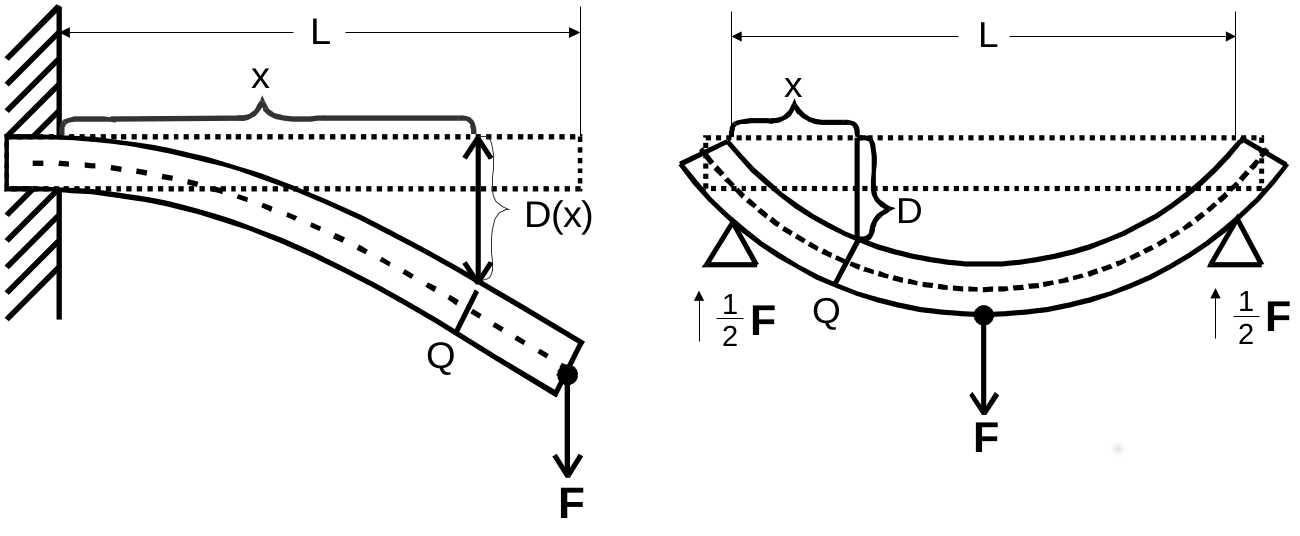
\includegraphics[scale=0.2]{content/Biegungen.png}
    \caption{Biegung eines einseitig eingespannten Stabes links.\newline
    Biegung eines beidseitig eingespannten Stabes rechts. [1]}
    \label{fig:abb1}
\end{figure}

Bei den dargestellten Biegungen handelt es sich um die Biegungen eines einseitig
eingespannten und eines beidseitig aufgelegten Stabes.

\subsection{Die Biegung eines Stabes bei einseitiger Einspannung}

Die am uneingespannten Ende des Stabes wirkende Gravitationskraft $F$ eines 
aufgehängten Gewichtes, biegt den Stab mit der Durchbiegung $D(x)$ und
bewirkt ein angreifendes Drehmoment

\begin{equation*}
    M_\text{F} = F \cdot (L - x)
\end{equation*}

mit der Länge des Hebelarms $(L - x)$.

Dieses Drehmoment verursacht eine Dehnung der oberen und eine Stauchung
der unteren Stabschichten, sodass der Querschnitt $Q$ sich nicht mehr in vertikaler,
sondern in verdrehter Position befindet. Einzig die neutrale Faser in der Mitte
des Querschnitts $Q$ behält ihre Länge bei. An allen anderen Fasern kommt es,
aufgrund der Elastizitäts des Körpers, zu Normalspannungen, die sich zu einem
zu $M_\text{F}$ entgegengesetzen Drehmoment $M_\sigma$ aufsummieren:

\begin{equation*}
    M_\sigma = \int_Q y \sigma(y) \; \symup{d}q
\end{equation*}

Dabei beschreibt $y$ den Abstand des Flächenelements $\symup{d}q$ zur neutralen Faser.

Zwischen den Drehmomenten stellt sich ein Gleichgewicht mit fester
Durchbiegung $D(x)$ ein, sodass 

\begin{align*}
    M_\text{F} &= M_\sigma \\
    \iff \; \int_Q y \sigma(y) \; \symup{d}q &= F \cdot (L - x)
\end{align*}

gilt.

Damit ergibt sich für die Durchbiegung

\begin{equation}
    D(x) = \frac{F}{2 E \symbf{I}} \left(L x^2 - \frac{x^3}{3} \right) 
    \qquad (\text{für } 0 \leq x \leq L)
    \label{eqn:Biegung}
\end{equation}

mit dem Flächenträgheitsmoment

\begin{equation}
    \symbf{I} = \int_Q y^2 \; \symup{d} q(y)
    \label{eqn:Traegheit}
\end{equation}

\subsection{Die Biegung eines Stabes mit beideitiger Auflage}

Am beidseitig aufgelegten Stab wirkt nach Abblidung \ref{fig:abb1} die Gravitationskraft
$\frac{F}{2}$ eines Gewichtes an der Mitte der Querschnittsfläche $Q$ mit einem
Hebelarm der Länge $x$ und bewirkt somit das Drehmoment

\begin{align*}
    M_\text{F} &= - \frac{F}{2} x \qquad \qquad \; \; \,
    (\text{für } 0 \leq x \leq \frac{L}{2})\\
    M_\text{F} &= - \frac{F}{2} (L - x) \qquad (\text{für } \frac{L}{2} \leq x \leq L)
\end{align*}

Damit ergibt sich analog die Durchbiegung

\begin{align}
    D(x) &= \frac{F}{48 E \symbf{I}} \left(3 L^2 x - 4 x^3 \right) 
    \qquad \qquad \qquad \qquad \: (\text{für } 0 \leq x \leq \frac{L}{2}) \\
    D(x) &= \frac{F}{48 E \symbf{I}} \left(4 x^3 - 12 L x^2 + 9 L^2 x - L^3 \right) 
    \qquad (\text{für } \frac{L}{2} \leq x \leq L)
    \label{eqn:Beidseitig}
\end{align}

\subsection{Berechnung der Flächenträgheitsmomente}

Das Flächenträgheitsmoment $I$ ist durch \eqref{eqn:Traegheit} definiert. 
Für einen Stab mit quadratischem Querschnitt mit Kantenlänge $a$ ergibt 
sich demnach: 

\begin{equation}
I_Q = \int_\frac{-a}{2}^\frac{a}{2} \int_\frac{-a}{2}^\frac{a}{2} y² \symup{d}y \symup{d}z 
= \int_\frac{-a}{2}^\frac{a}{2} \frac{2}{3} \frac{a³}{8} \symup{d}z 
= a \cdot \frac{2}{3} \frac{a³}{8} 
= \frac{a⁴}{12}
\label{eqn:Quadratisch}
\end{equation}

Weiterhin ergibt sich für einen runden Stab mit Durchmesser $d$ unter 
Verwendung von Polarkoordinaten: 

\begin{align}
I_K &= \int_0^2\pi \int_0^\frac{d}{2} (r \cdot \sin(\varphi))²\cdot \symup{d}r \symup{d}\varphi
= \frac{1}{4}\left(\frac{d}{2}\right)⁴ \int_0^2\pi \sin(\varphi)² \symup{d}\varphi\\
&= \left.\frac{d⁴}{64} \frac{\varphi}{2} - \frac{\sin(\varphi) \cos{\varphi}}{2} \right|_0^2\pi
= \frac{\pi}{64} d⁴
\label{eqn:Rund}
\end{align}











